\documentclass[../AnalysisNoteJBuxton.tex]{subfiles}
\begin{document}

\subsection{Cascade Reconstruction}
\label{CascadeReconstruction}

A description of our $\Xi$K$^{\pm}$ analyses, as well as preliminary results and fits are expected to be uploaded by 16 December 2016.

Our motivation for studying $\Xi$K$^{\pm}$ systems is to hopefully better understand the striking difference in the $\Lambda$K$^{+}$ and $\Lambda$K$^{-}$ data at low $k^{*}$ (Figure \ref{fig:cLamcKchCfs0010}).

The reconstruction of $\Xi$ particles is one step above V0 reconstruction.  V0 particles are topologically reconstructed by searching for the charged daughters' tracks into which they decay.  With $\Xi$ particles, we search for the V0 particle and charged daughter into which the $\Xi$ decays.  In the case of $\Xi^{-}$, we search for the $\Lambda$ (V0) and $\pi^{-}$ (track) daughters.  We will refer to this $\pi$ as the ``bachelor $\pi$".  The reconstruction of $\Xi$, and the specific cuts used will be included in future versions of this note.

\begin{figure}[h]
  \centering
  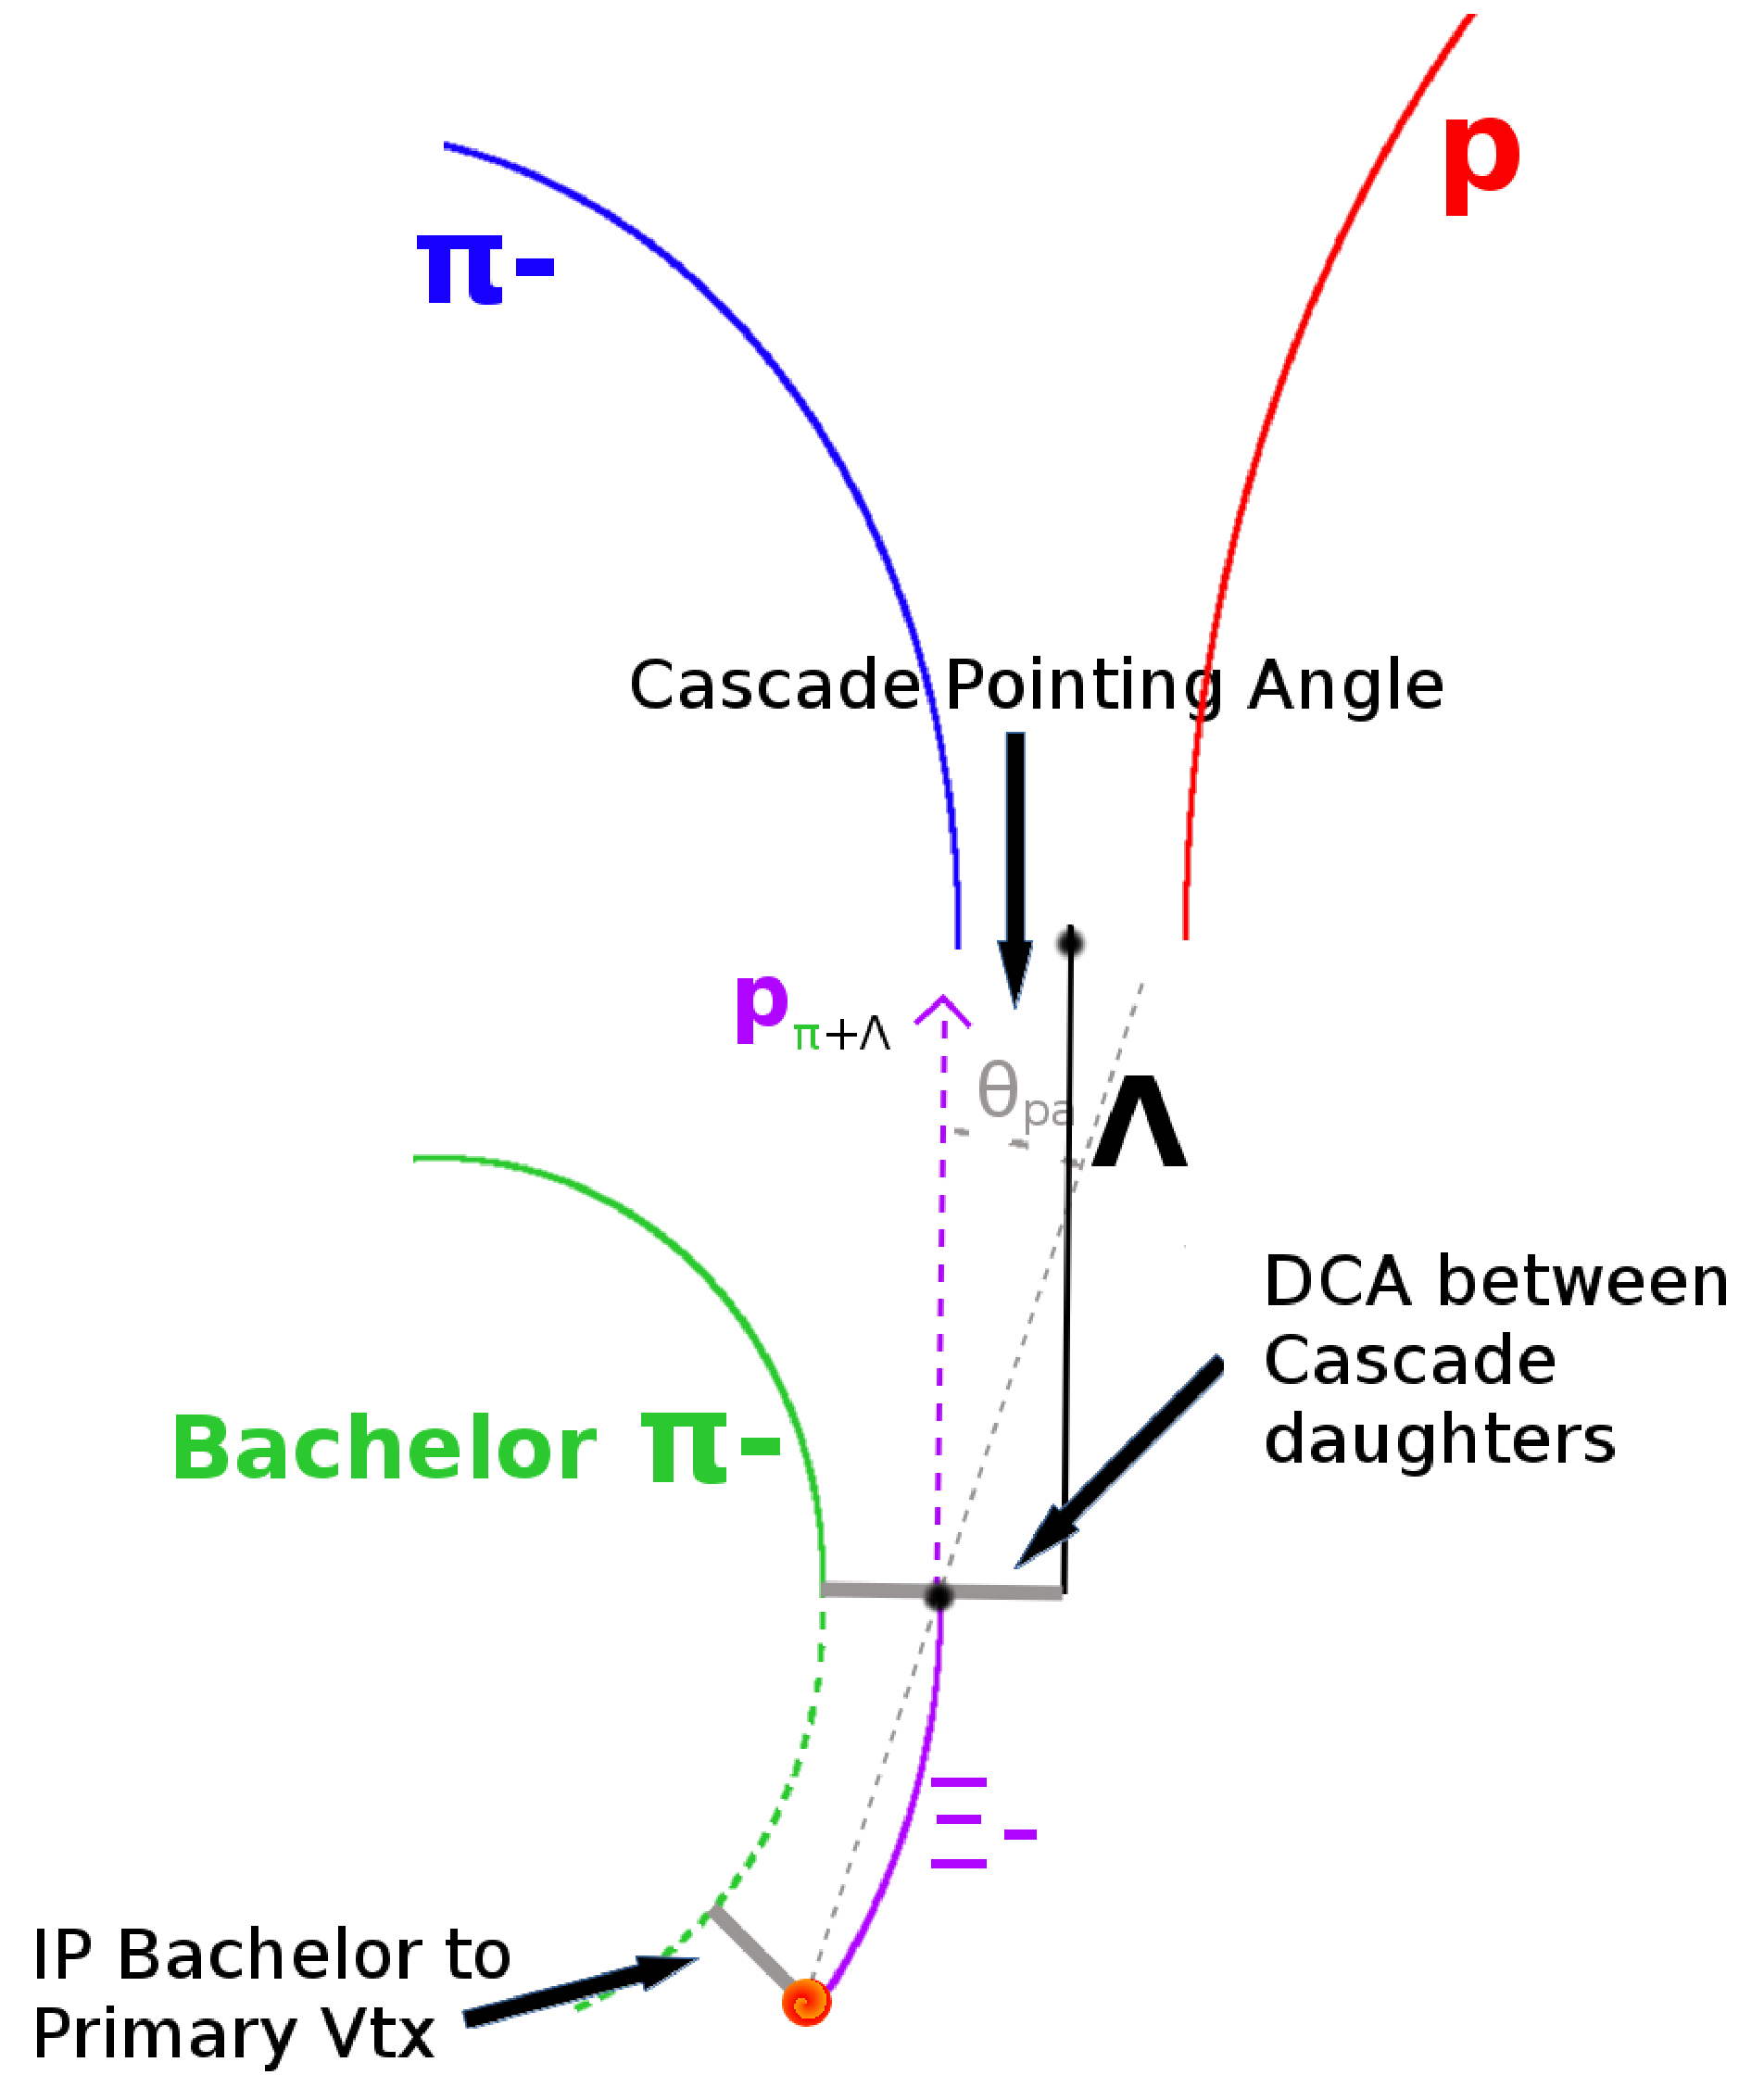
\includegraphics[width=0.5\textwidth]{3_DataSelection/Figures/XiCuts.pdf}
  \caption[$\Xi$ Reconstruction]{$\Xi$ Reconstruction}
  \label{fig:XiReconstruction}
\end{figure}

The purity of our $\Xi$ and $\bar{\Xi}$ collections are calculated just as those of our V0 collections \ref{V0Selection}.
Figure \ref{fig:XiPurity}, which is used to calculate the purity, shows the m$_{inv}$ distribution of our $\Xi$($\bar{\Xi}$) candidates just before the final m$_{inv}$ cut.  Currently, we have Purity($\Xi^{-}$) $\approx$ 81\% and Purity($\bar{\Xi}^{+}$) $\approx$ 86\%.

\begin{figure}[h!]
  \centering
  %%----start of first subfigure---  
  \subfloat[$\Xi^{-}$ Purity]{
    \label{fig:XiPurity:a}
    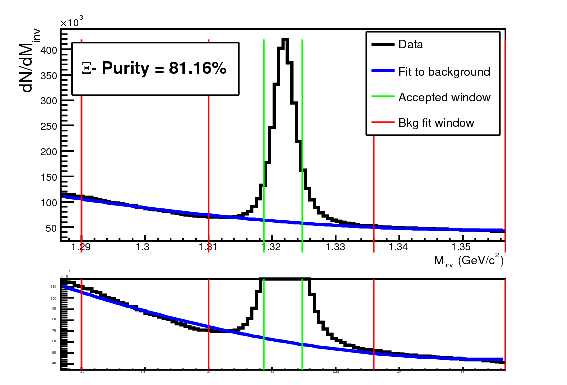
\includegraphics[width=0.49\textwidth]{3_DataSelection/Figures/XiPurity_XiKchP.pdf}}
  %%----start of second subfigure---
  \subfloat[$\bar{\Xi}$ Purity]{
    \label{fig:XiPurity:b}
    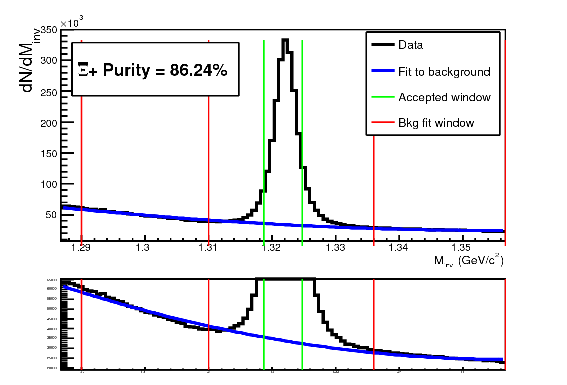
\includegraphics[width=0.49\textwidth]{3_DataSelection/Figures/AXiPurity_XiKchP.pdf}}
  %%----overall caption----
  \caption[$\Xi^{-}$($\bar{\Xi}^{+}$) Purity]{$\Xi^{-}$($\bar{\Xi}^{+}$) Purity:  Currently, we have Purity($\Xi^{-}$) $\approx$ 81\% and Purity($\bar{\Xi}^{+}$) $\approx$ 86\%.}
  \label{fig:XiPurity}
\end{figure}

\end{document}